\section{Hierarchie des pages}
			Voici l'arborescence "ressentie" par l'utilisateur :
			
		\section{Contenu}
			\subsection{Le Menu}

	Le menu a 4 liens principaux : 
	\begin{description}
		\item[Acheter :] Renvoie vers les catégories de produits achetables.
		\item[Louer :] Renvoie vers les catégories de produits louables.
		\item[A Propos :] Affichage d'informations relatives à Brico-Bob.
		\item[Contact :] Affiche les coordonnées des administrateurs du site\\
		 ( et du service 	client par exemple ).
	\end{description}

	Le menu est aussi déroulant lorsque l'utilisateur survole "Acheter" et "Louer", 	ce qui lui permet d'accéder directement aux catégories de produits.
	
	\subsection{Catégories - Sous catégories}

	Une catégorie ou une sous catégorie peut contenir soit d'autre catégories, 	soit des produits. Il est donc techniquement avoir une arborescence comme ceci par exemple :

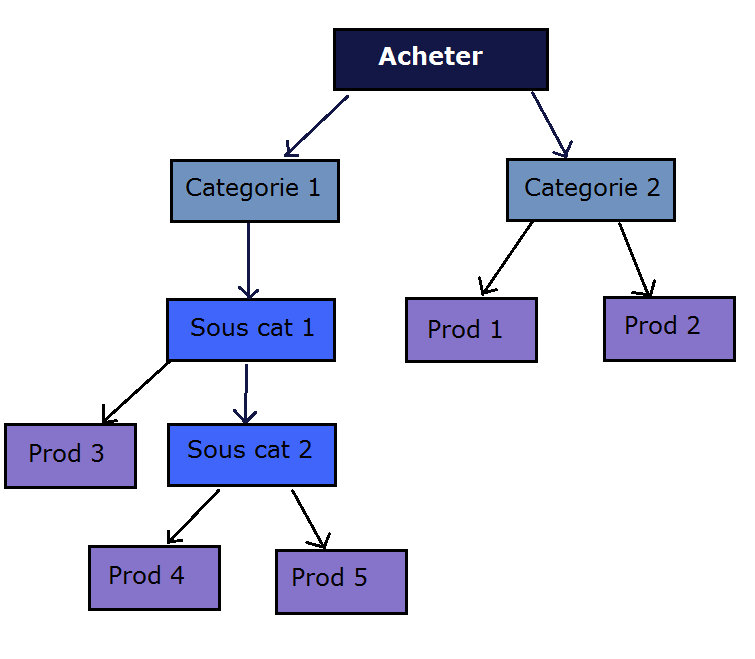
\includegraphics[scale=0.7]{arbocatego.png}

	\subsection{Fiche produit}

	La fiche produit contiens les informations relatives au produit, les liens pour l'acheter ou le louer, et les avis des utilisateurs.
Chaque utilisateur peut ajouter un commentaire et "noter le produit", un peu comme sur un blog. Le formulaire d'ajout d'un commentaire se trouve en
bas de la page fiche produit. 
		
	\subsection{Coups de cœur}

	Les coups de cœur sur la page d'accueil représentent des produits à mettre en valeur, qui sont par exemple le dernier produit ajouté dans la base de donnée afin d'en assurer sa promotion
		
	\subsection{Panneau d'administration}

	Lorsque l'administrateur se connecte, il a accès au panneau d'administration. Ce panneau lui permet plusieurs choses comme cela est expliqué :
	
	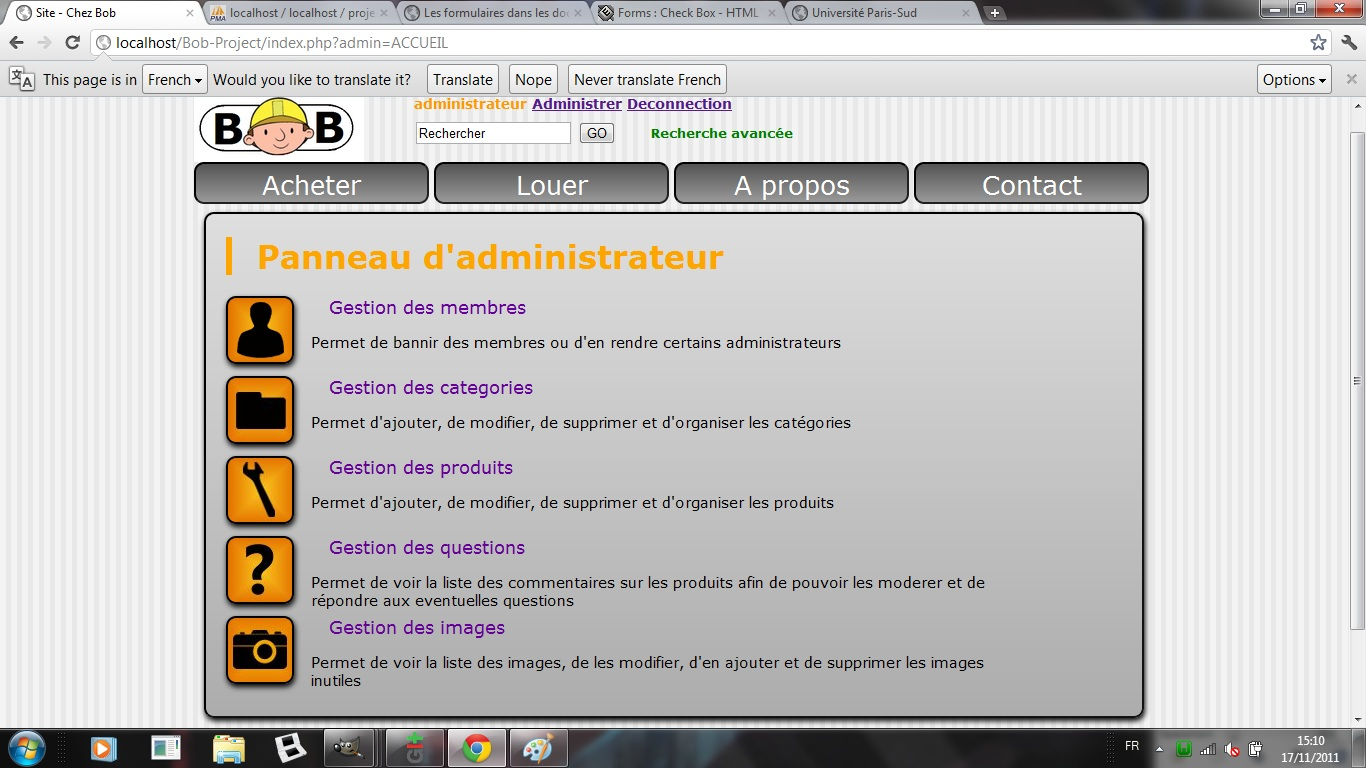
\includegraphics[scale=0.5]{panneauadmin.jpg}
			
		\section{Des pages, un design}	
			Nous avons utilisé des fichiers .css pour quasiment toute la mise en forme du site. Le seul endroit ou nous avons utilisé un tableau est la gestion des membres dans le panneau administrateur. Voila une liste non exhaustive des écrans de notre site avec les différentes "boites".
					
			
		\section{Un formulaire}
			Les formulaires sont pour la plupart de type POST, seuls ceux de recherche sont de type GET pour pouvoir, à partir du lien refaire la recherche.\\
			Alors que les pages sont généralement appellées avec \$\_GET["page"], les formulaires appellent index.php avec \$\_GET["action"].\\
			Pour se connecter, on cliquera sur le lien : index.php?page=CONNEXION et le formulaire (qui s'y trouve) appelle index.php?action=CONNEXION
		\section{La sécurité}
			Certains formulaires sont controles par JavaScript (avec Ajax, parfois), mais le réel controle se situe au niveau du php.\\
			Les informations que le client entre sont sécurisées pour la faille XSS, mais pas celles des admins, qui ont loisir d'injecter des scripts CSS/HTML/JavaScript sur certaines descriptions.\\
			Nous estimons que l'administrateur est digne de confiance pour ne pas tenter de prendre des informations du site sur un serveur distant.